\section{Stage II: Where the Remaining Time Goes}
\label{sec:stage2}

\subsection{Region Profiling}
\label{sec:regions}
flambda2 inlines the whole forward pass into one symbol, which a sampling
profiler cannot split, so I wrote a region profiler
(\code{tools/profile_regions.py}) that instruments the C++ and OCaml ports at
identical region boundaries with the time-stamp counter. The counters perturb
the compilers differently (scalar C++ lost 9.8\% throughput, OxCaml 5.2.0+ox
6.7\%), so each region's \emph{share} comes from the instrumented run and the
total from the uninstrumented binary. The regions cover 97--100\% of the
forward pass.

\begin{figure}[h]
  \centering
  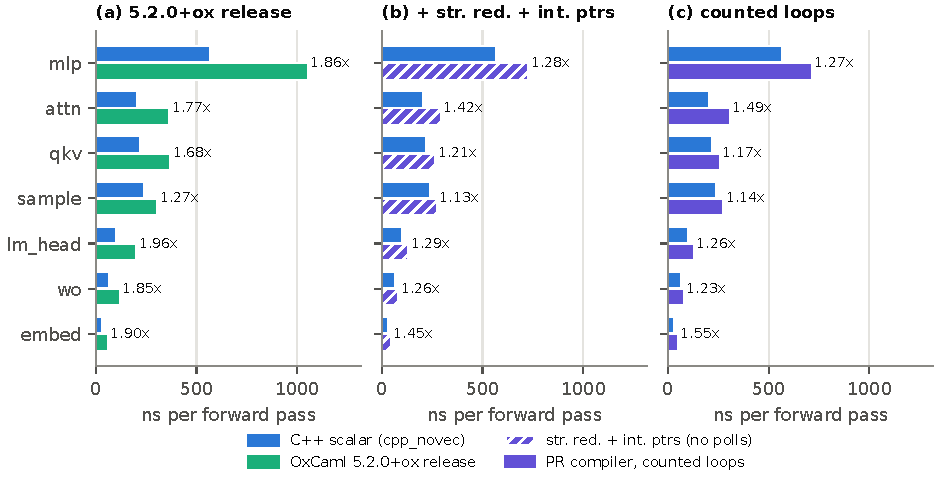
\includegraphics[width=\textwidth]{fig_regions}
  \caption{Nanoseconds per forward pass by region against scalar C++
  (1,431\,ns per token), separate region-profile run (7 rounds); labels give
  the OCaml/C++ ratio. (a) OxCaml 5.2.0+ox release, unrolled kernel:
  2,471\,ns ($1.73\times$). (b) Strength reduction and interior pointers, no
  polls (Section~\ref{sec:ip}): 1,815\,ns ($1.27\times$). (c) Counted loops,
  polls at loop exits (Section~\ref{sec:counted}): 1,810\,ns ($1.26\times$).}
  \label{fig:regions}
\end{figure}

No single region is pathological. The four regions dominated by \code{linear}
(\code{mlp}, \code{qkv}, \code{lm_head}, \code{wo}) run at similar ratios,
$1.69$--$1.95\times$ (C++ about 0.25\,ns per multiply--add, OxCaml about
0.47), and account for 75\% of the gap; \code{sample}, which spends much of
its time in the same C library \code{exp}, is closest ($1.27\times$). The
bottleneck is \code{linear}'s inner loop.

\subsection{The Gap Is Not SIMD}
The shipped C++ kernel contains 27 packed SSE2 instructions; OxCaml emits only
scalar arithmetic. Yet GCC's vectoriser is worth only
$+9.5\%$ (21/21) to C++, and scalar C++ is still
$1.65\times$ faster than OxCaml. The gap is scalar overhead around
the arithmetic.

\subsection{The Hot Loop, Instruction by Instruction}
\label{sec:hotloop}

\begin{lstlisting}[language=asmX,caption={OxCaml 5.2.0+ox, where this work began, unrolled kernel: 23 instructions per 4 MACs.},label=lst:ox-hot]
vmovsd -0x4(%rax,%rbp,4),%xmm4        # x.(i)
mov    %r9,%r10                       # rebuild b0 + i ...
add    %rbp,%r10                      # ... every iteration
vmulsd -0x8(%rbx,%r10,4),%xmm4,%xmm5  # d.(b0+i), load folded into the multiply
vaddsd %xmm5,%xmm3,%xmm3
mov    (%rsp),%r10                    # b1 was spilled: reload it
add    %rbp,%r10
vmulsd -0x8(%rbx,%r10,4),%xmm4,%xmm5
vaddsd %xmm5,%xmm2,%xmm2
# ... rows 2 and 3: the same mov / add / vmulsd / vaddsd ...
cmp    %r13,%rbp                      # exit test before the increment
je     .Lexit
add    $0x2,%rbp                      # i++ (tagged, step 2)
cmp    (%r14),%r15                    # GC safepoint poll
jbe    .Lgc
jmp    .Ltop                          # extra unconditional back edge
\end{lstlisting}

\begin{lstlisting}[language=asmX,caption={C++ with \texttt{-fno-tree-vectorize}: 15 instructions per 4 MACs.},label=lst:cpp-hot]
movsd  (%rcx,%rax), %xmm0     # x[i]
movsd  (%rdi,%rax), %xmm5     # w0[i]
mulsd  %xmm0, %xmm5
addsd  %xmm5, %xmm4
movsd  (%rsi,%rax), %xmm5     # w1[i]
mulsd  %xmm0, %xmm5
addsd  %xmm5, %xmm3
movsd  (%rdx,%rax), %xmm5     # w2[i]
mulsd  %xmm0, %xmm5
mulsd  (%r8,%rax), %xmm0      # w3[i]
addq   $8, %rax               # ONE offset advances all four rows
addsd  %xmm5, %xmm2
addsd  %xmm0, %xmm1
cmpq   %rax, %r9
jne    .L13
\end{lstlisting}

Both inner loops (Listings~\ref{lst:ox-hot} and~\ref{lst:cpp-hot}) do the same
8 floating-point operations; the 5.4.0-ox7 release emits the same loop
structure (21 instructions including the poll). The difference is integer
bookkeeping, with five sources:

\begin{enumerate}
  \item \textbf{No interior pointers} (8 instructions): OCaml rebuilds
        \code{b_k + i} for every row on every iteration, where C++ keeps four
        row pointers and one shared offset.
  \item \textbf{A register spill} (one of those 8 is a stack load): with
        \reg{r14} and \reg{r15} reserved and \reg{r11} unavailable across the
        poll, one row base lives on the stack.
  \item \textbf{The safepoint poll} (2 instructions), although the loop
        neither allocates nor calls.
  \item \textbf{Loop shape} (1 extra instruction): the poll block forces an
        unconditional \code{jmp}.
  \item \textbf{Tagging}, which costs nothing: scale-4 addressing absorbs it.
\end{enumerate}

Figure~\ref{fig:budget} summarises the budget and where the compiler work of
Sections~\ref{sec:sr}--\ref{sec:ip} takes the loop. The instruction ratio,
23/15 = $1.53\times$, is of the same size as the measured gap
($1.65\times$ on the release), but one counts the inner loop alone and the other
times the whole program, about a quarter of whose gap lies outside
\code{linear}.

\begin{figure}[h]
  \centering
  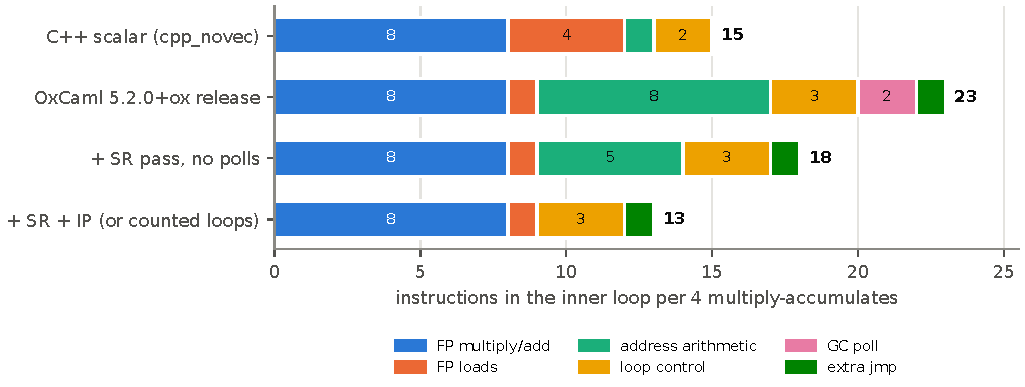
\includegraphics[width=0.9\textwidth]{fig_budget}
  \caption{Inner-loop instructions per four multiply--accumulates. The two
  lower rows are the passes of Sections~\ref{sec:sr} and~\ref{sec:ip} on a
  compiler configured without polls; with polls on, counted loops give the
  same 13-instruction loop.}
  \label{fig:budget}
\end{figure}

The first cause belongs to the language and its collector; the second to fourth
to the compiler.
